% ===========================================================================
% Évaluer des arbres de décision
% Traduit et adapté de :
%   https://www.bootstrapworld.org/materials/fall2026/en-us/lessons/decision-trees-evaluating/
% Suite de la leçon « Construire des arbres de décision »
% Licence : Creative Commons 4.0 Unported (Bootstrap Community)
% ===========================================================================

\documentclass[12pt,a4paper]{article}

% ---------- Packages ----------
\usepackage[utf8]{inputenc}
\usepackage[T1]{fontenc}
\usepackage{libertine}
\usepackage{microtype}
\usepackage[french]{babel}
\usepackage{graphicx}
\usepackage{float}
\usepackage{hyperref}
\usepackage{geometry}
\usepackage{enumitem}
\usepackage{tabularx}
\usepackage{xcolor}
\usepackage[raster]{tcolorbox}
\usepackage{booktabs}
\usepackage{colortbl}
\usepackage{fancyhdr}
\usepackage{titlesec}
\usepackage{amsmath}
\usepackage{amssymb}
\usepackage{listings}
\usepackage{tikz}
\usetikzlibrary{trees, arrows.meta, positioning, shapes.geometric, calc, matrix}

% ---------- Mise en page ----------
\geometry{margin=2.5cm, headheight=15pt, footskip=30pt}
\fancyhf{}
\fancyhead[L]{\textbf{Évaluer des arbres de décision}}
\fancyhead[R]{\thepage}
\fancyfoot[C]{Bootstrap Community — CC BY 4.0}
\renewcommand{\headrulewidth}{0.4pt}
\pagestyle{fancy}

% ---------- Couleurs ----------
\definecolor{bsblue}{RGB}{41,128,185}
\definecolor{bsgreen}{RGB}{39,174,96}
\definecolor{bsorange}{RGB}{230,126,34}
\definecolor{bsgray}{RGB}{149,165,166}
\definecolor{codebg}{RGB}{245,247,250}
\definecolor{leafgreen}{RGB}{39,174,96}
\definecolor{nodeorange}{RGB}{230,126,34}
\definecolor{rootblue}{RGB}{41,128,185}
\definecolor{tp}{RGB}{39,174,96}      % True Positive  - vert
\definecolor{tn}{RGB}{41,128,185}     % True Negative  - bleu
\definecolor{fp}{RGB}{230,126,34}     % False Positive - orange
\definecolor{fn}{RGB}{192,57,43}      % False Negative - rouge

% ---------- Styles de sections ----------
\titleformat{\section}[hang]{\Huge\bfseries\color{bsblue}}{}{0pt}{}[\vspace{-0.5em}\rule{\textwidth}{2pt}]
\titleformat{\subsection}[hang]{\Large\bfseries\color{bsblue!80!black}}{}{0pt}{}
\titleformat{\subsubsection}[hang]{\large\bfseries\color{bsgreen!60!black}}{}{0pt}{}

% ---------- Environnements personnalisés ----------
\newtcolorbox{overviewbox}{
  colback=bsblue!5!white, colframe=bsblue!60!white,
  fonttitle=\bfseries, title=Objectif de la section,
  left=1em, right=1em, top=0.5em, bottom=0.5em
}
\newtcolorbox{activitybox}{
  colback=bsgreen!5!white, colframe=bsgreen!60!white,
  fonttitle=\bfseries, title=Activité,
  left=1em, right=1em, top=0.5em, bottom=0.5em
}
\newtcolorbox{thinkbox}{
  colback=bsorange!5!white, colframe=bsorange!60!white,
  fonttitle=\bfseries, title=Réflexion,
  left=1em, right=1em, top=0.5em, bottom=0.5em
}
\newtcolorbox{keypointbox}{
  colback=bsgray!10!white, colframe=bsgray!50!white,
  fonttitle=\bfseries, title=Point clé,
  left=1em, right=1em, top=0.5em, bottom=0.5em
}
\newtcolorbox{instructornotes}{
  colback=yellow!10!white, colframe=yellow!80!black,
  fonttitle=\bfseries, title=Notes pour l'enseignant·e,
  left=1em, right=1em, top=0.5em, bottom=0.5em
}
\newtcolorbox{codebox}{
  colback=codebg, colframe=bsgray!40,
  fonttitle=\bfseries, title=Code Pyret,
  left=1em, right=1em, top=0.5em, bottom=0.5em
}
\newtcolorbox{contractbox}{
  colback=bsblue!3!white, colframe=bsblue!40!white,
  left=1em, right=1em, top=0.6em, bottom=0.6em
}

% ---------- Style listings pour Pyret ----------
\lstdefinelanguage{Pyret}{
  keywords={use,context,url-file,and,or,not,if,else,for,fun,data,sharing,include,import,as,where,let,rec,is,=,true,false,load-table,source,end,Row,String,Number,Boolean,Table,Image,DecisionTree,List,build-tree,confusion-matrix,classify,image-dot-plot,dt-code},
  sensitive=true,
  comment=[l]{\#},
  morestring=[b]",
  morestring=[b]',
}
\lstset{
  language=Pyret,
  basicstyle=\ttfamily\small,
  commentstyle=\color{bsgreen!70!black}\itshape,
  keywordstyle=\color{bsblue}\bfseries,
  stringstyle=\color{bsorange},
  backgroundcolor=\color{codebg},
  frame=single,
  framesep=5pt,
  rulecolor=\color{bsgray!40},
  breaklines=true,
  breakatwhitespace=false,
  showstringspaces=false,
  aboveskip=0.8em,
  belowskip=0.8em,
}

% ---------- Commandes pratiques ----------
\newcommand{\img}[3]{%
  \begin{figure}[H]
    \centering
    \includegraphics[#2]{#1}
    \caption{#3}
    \label{fig:#1}
  \end{figure}
}
\newcommand{\contrat}[1]{%
  \begin{contractbox}
    \ttfamily #1
  \end{contractbox}
}

% ---------- Arbre de décision TikZ ----------
\tikzset{
  root/.style={draw=rootblue, thick, fill=rootblue!15, rounded corners=4pt,
               align=center, font=\small\bfseries, text=rootblue, inner sep=4pt, minimum width=2.8cm},
  decision/.style={draw=nodeorange, thick, fill=nodeorange!10, rounded corners=4pt,
                   align=center, font=\small\bfseries, text=nodeorange!80!black, inner sep=4pt, minimum width=2.8cm},
  leaf/.style={draw=leafgreen, thick, fill=leafgreen!10, rounded corners=4pt,
               align=center, font=\small\bfseries, text=leafgreen!70!black, inner sep=4pt, minimum width=2.5cm},
  split-yes/.style={->, >=Stealth, thick, draw=bsgreen, font=\scriptsize\bfseries},
  split-no/.style={->, >=Stealth, thick, draw=bsorange, font=\scriptsize\bfseries},
}

% ---------- Informations du document ----------
\title{%
  \vspace{-2cm}
  {\Huge\bfseries Évaluer des}\\[0.3em]
  {\Huge\bfseries arbres de décision}\\[0.5em]
  {\large Surapprentissage, matrices de confusion et limites des classificateurs}\\[1em]
  {\normalsize Traduit et adapté depuis \href{https://www.bootstrapworld.org/materials/fall2026/en-us/lessons/decision-trees-evaluating/}{Bootstrap World} (Fall 2026)}\\
  {\normalsize Suite de la leçon «~Construire des arbres de décision~»}\\[0.5em]
  {\normalsize Licence Creative Commons 4.0 International}
}
\date{}
\author{}

\begin{document}

\maketitle
\thispagestyle{empty}

\vspace{2cm}
\begin{center}
  \textit{Ces supports ont été développés en partie grâce au soutien de la National Science Foundation\\
  (bourses 1042210, 1535276, 1648684, 1738598, 2031479 et 1501927).}
\end{center}

\newpage
\tableofcontents
\newpage

% ===========================================================================
% SECTION 1 : CONSTRUIRE DES ARBRES DE DÉCISION EN PYRET
% ===========================================================================
\section{Construire des arbres de décision en Pyret}

\begin{overviewbox}
  Maintenant que les élèves connaissent l'algorithme de construction d'un arbre de décision, iels explorent la capacité de Pyret à construire des arbres \emph{automatiquement}. Iels étudient l'impact de la profondeur maximale et du choix des colonnes sur la qualité d'un classificateur.
\end{overviewbox}

% ---------- Launch ----------
\subsection{Lancement}

Récapitulons ce que nous savons sur les classificateurs~:

\begin{itemize}
  \item Il existe un algorithme simple pour calculer un \emph{arbre optimal} pour n'importe quel jeu de données.
  \item Les arbres de décision sont en réalité des fonctions appelées \emph{classificateurs}~: iels prennent une entrée et produisent une prédiction.
  \item Tous les arbres de décision ne se valent pas~!
\end{itemize}

Bien sûr, calculer un arbre de décision à la main prend beaucoup de temps, surtout s'il y a des dizaines de milliers de lignes et des centaines de colonnes~! Heureusement, les ordinateurs sont \emph{vraiment, vraiment} doués pour suivre des algorithmes.

\begin{keypointbox}
  Un exemple d'application précoce de ce type d'automatisation est utilisé par la \textbf{United States Postal Service} (service postal des États-Unis) pour lire les adresses manuscrites sur les enveloppes. Leur système d'interprétation d'adresses a été entraîné sur la base de données \textbf{MNIST} (\emph{Modified National Institute of Standards and Technology}), qui contient des milliers d'images étiquetées de chiffres manuscrits.
\end{keypointbox}

% ---------- Investigate ----------
\subsection{Exploration~: \texttt{build-tree}}

Étant donné un jeu de données sur lequel s'entraîner, Pyret peut construire des arbres de décision \emph{optimaux} pour nous, et même nous donner le code du classificateur correspondant — en utilisant exactement l'algorithme que vous connaissez déjà~!

\contrat{\# build-tree :: (Table t, List<String> colonnes, String colonne-reponse, Number profondeur-max) -> DecisionTree}

La fonction \texttt{build-tree} prend \textbf{quatre arguments} dans son Domaine~:
\begin{enumerate}[leftmargin=*]
  \item Le \emph{jeu de données d'entraînement} sur lequel ajuster l'arbre.
  \item Une \emph{liste de noms de colonnes} sur lesquelles les nœuds peuvent se diviser.
  \item Le nom de la \emph{colonne cible} contenant les «~réponses~» (les catégories à prédire).
  \item La \emph{profondeur maximale} autorisée pour l'arbre.
\end{enumerate}

\subsubsection{Construire des arbres à un niveau}

\begin{activitybox}
  Dans la Zone de Définitions, définissez \texttt{tree-c1} comme un arbre à 1~niveau utilisant uniquement la colonne catégorielle \texttt{"queue"}, puis cliquez sur «~Run~»~:
  \begin{lstlisting}
tree-c1 = build-tree(training, [list: "queue"], "espece", 1)
  \end{lstlisting}

  \begin{enumerate}[leftmargin=*]
    \item Évaluez \texttt{tree-c1}. Si un animal n'a pas de queue, que prédit-il~?
    \item Évaluez \texttt{dt-code(tree-c1)}. Où avez-vous déjà vu ce code~?
    \begin{itemize}
      \item C'est la même fonction que \texttt{classifieur-queue}, déjà présente dans notre Zone de Définitions~!
    \end{itemize}
  \end{enumerate}

  Définissez maintenant \texttt{tree-q1} comme un arbre à 1~niveau utilisant uniquement la colonne quantitative \texttt{"poids"}, puis cliquez sur «~Run~»~:
  \begin{lstlisting}
tree-q1 = build-tree(training, [list: "poids"], "espece", 1)
  \end{lstlisting}

  \begin{enumerate}[leftmargin=*, resume]
    \item Évaluez \texttt{tree-q1}. Quelle division Pyret a-t-il trouvée~?
    \begin{itemize}
      \item Il a trouvé qu'il était plus pertinent de diviser à \textbf{9,55~kg}~!
    \end{itemize}
  \end{enumerate}

  Définissez \texttt{tree-any1} comme un arbre à 1~niveau autorisé à utiliser \emph{n'importe quelle} colonne~:
  \begin{lstlisting}
tree-any1 = build-tree(training, [list: "sexe", "queue", "mammifere", "nage", "poids"], "espece", 1)
  \end{lstlisting}

  \begin{enumerate}[leftmargin=*, resume]
    \item Quelle colonne \emph{auriez-vous} choisie pour le nœud racine~? Évaluez \texttt{tree-any1}. Quelle colonne \emph{Pyret} a-t-il choisie~?
    \begin{itemize}
      \item \texttt{"nage"} — c'est la colonne qui sépare le mieux les données.
    \end{itemize}
  \end{enumerate}
\end{activitybox}

\subsubsection{Construire des arbres à plusieurs niveaux}

\begin{activitybox}
  Ajoutez les définitions suivantes à la Zone de Définitions et cliquez sur «~Run~»~:
  \begin{lstlisting}
tree-c2   = build-tree(training, [list: "queue"], "espece", 2)
tree-q2   = build-tree(training, [list: "poids"], "espece", 2)
tree-any2 = build-tree(training, [list: "sexe", "queue", "mammifere", "nage", "poids"], "espece", 2)
  \end{lstlisting}

  \begin{enumerate}[leftmargin=*]
    \item Dans le code ci-dessus, nous avons autorisé \texttt{tree-c2} à avoir une profondeur maximale de~2. L'arbre résultant n'a en fait qu'\emph{un} niveau. Pourquoi~?
    \begin{itemize}
      \item Une fois qu'on a divisé sur \texttt{queue}, il n'y a plus rien à trier avec \emph{seulement} la colonne \texttt{"queue"}.
    \end{itemize}
    \item En quoi les arbres \texttt{tree-c1} et \texttt{tree-c2} sont-ils différents~? Identiques~?
    \begin{itemize}
      \item Ils sont identiques~! La colonne \texttt{queue} ne permet qu'une seule division utile.
    \end{itemize}
  \end{enumerate}

  Ajoutez maintenant~:
  \begin{lstlisting}
tree-q3   = build-tree(training, [list: "poids"], "espece", 3)
tree-q4   = build-tree(training, [list: "poids"], "espece", 4)
tree-q5   = build-tree(training, [list: "poids"], "espece", 5)
tree-any3 = build-tree(training, [list: "sexe", "queue", "mammifere", "nage", "poids"], "espece", 3)
tree-any4 = build-tree(training, [list: "sexe", "queue", "mammifere", "nage", "poids"], "espece", 4)
tree-any5 = build-tree(training, [list: "sexe", "queue", "mammifere", "nage", "poids"], "espece", 5)
  \end{lstlisting}

  \begin{enumerate}[leftmargin=*, resume]
    \item Comparez \texttt{tree-q1}, \texttt{tree-q2} et \texttt{tree-q3}. En quoi sont-ils similaires~? Différents~?
    \begin{itemize}
      \item Ils commencent tous par \emph{la même division} (poids $< 9{,}55$), mais gagnent en profondeur pour mieux séparer les espèces.
    \end{itemize}
  \end{enumerate}
\end{activitybox}

% Diagrammes ASCII en codebox pour tree-q1, tree-q2, tree-q3
\begin{codebox}
Les trois arbres \texttt{tree-q1}, \texttt{tree-q2} et \texttt{tree-q3} construits uniquement sur la colonne \texttt{"poids"}~:
\end{codebox}

\begin{center}
\begin{tikzpicture}[
  every node/.style={align=center, font=\scriptsize},
  level 1/.style={sibling distance=2.3cm, level distance=1.1cm},
  level 2/.style={sibling distance=1.6cm, level distance=1.1cm},
  level 3/.style={sibling distance=1.2cm, level distance=1.0cm},
  edge from parent/.style={draw, thick, ->, >=Stealth},
  qroot/.style={draw=rootblue, thick, fill=rootblue!15, rounded corners=3pt, font=\scriptsize\bfseries, text=rootblue, inner sep=2pt, minimum width=1.8cm},
  qdec/.style={draw=nodeorange, thick, fill=nodeorange!10, rounded corners=3pt, font=\scriptsize\bfseries, text=nodeorange!80!black, inner sep=2pt, minimum width=1.8cm},
  qleaf/.style={draw=leafgreen, thick, fill=leafgreen!10, rounded corners=3pt, font=\scriptsize\bfseries, text=leafgreen!70!black, inner sep=2pt, minimum width=1.3cm},
]
\matrix[column sep=2.5em] {
\begin{scope}
\node[qroot] {poids $< 9{,}55$~?}
  child {node[qleaf] {chat} edge from parent node[left, font=\tiny, text=bsgreen] {oui}}
  child {node[qleaf] {chien} edge from parent node[right, font=\tiny, text=bsorange] {non}};
\end{scope}
&
\begin{scope}
\node[qroot] {poids $< 9{,}55$~?}
  child {node[qdec] {poids $< 0{,}19$~?}
    child {node[qleaf] {escargot}  edge from parent node[left, font=\tiny, text=bsgreen] {oui}}
    child {node[qleaf] {chat}      edge from parent node[right, font=\tiny, text=bsorange] {non}}
    edge from parent node[left, font=\tiny, text=bsgreen] {oui}
  }
  child {node[qleaf] {chien}         edge from parent node[right, font=\tiny, text=bsorange] {non}};
\end{scope}
&
\begin{scope}
\node[qroot] {poids $< 9{,}55$~?}
  child {node[qdec] {poids $< 0{,}19$~?}
    child {node[qleaf] {escargot}  edge from parent node[left, font=\tiny, text=bsgreen] {oui}}
    child {node[qdec] {poids $< 1{,}95$~?}
      child {node[qleaf] {tarentule}  edge from parent node[left, font=\tiny, text=bsgreen] {oui}}
      child {node[qleaf] {chat}       edge from parent node[right, font=\tiny, text=bsorange] {non}}
      edge from parent node[right, font=\tiny, text=bsorange] {non}
    }
    edge from parent node[left, font=\tiny, text=bsgreen] {oui}
  }
  child {node[qleaf] {chien}         edge from parent node[right, font=\tiny, text=bsorange] {non}};
\end{scope}
\\
\node[font=\scriptsize\bfseries, below=2pt, text=bsblue] {tree-q1};
&
\node[font=\scriptsize\bfseries, below=2pt, text=bsblue] {tree-q2};
&
\node[font=\scriptsize\bfseries, below=2pt, text=bsblue] {tree-q3};
\\
};
\end{tikzpicture}
\end{center}

\subsection{Comparer les arbres}

\begin{activitybox}
  Assurez-vous d'avoir enregistré toutes les nouvelles définitions dans votre copie du fichier \texttt{Arbre-Decision-Starter.arr}. Évaluez chaque arbre et utilisez la fonction \texttt{classify} pour compter combien d'animaux du jeu d'entraînement sont correctement classifiés.

  \begin{center}
  \begin{tabularx}{\textwidth}{l c c X X}
    \toprule
    \textbf{arbre} & \textbf{niv. max} & \textbf{niv. réels} & \textbf{\# correct (entraînement)} & \textbf{\# correct (test)} \\
    \midrule
    \texttt{tree-c1}   & 1 & 1 & & \\
    \texttt{tree-q1}   & 1 & 1 & & \\
    \texttt{tree-any1} & 1 & 1 & & \\
    \texttt{tree-c2}   & 2 &   & & \\
    \texttt{tree-q2}   & 2 &   & & \\
    \texttt{tree-any2} & 2 &   & & \\
    \texttt{tree-q3}   & 3 &   & & \\
    \texttt{tree-any3} & 3 &   & & \\
    \texttt{tree-q4}   & 4 &   & & \\
    \texttt{tree-any4} & 4 &   & & \\
    \texttt{tree-q5}   & 5 &   & & \\
    \texttt{tree-any5} & 5 &   & & \\
    \texttt{tree-q6}   & 6 &   & & \\
    \bottomrule
  \end{tabularx}
  \end{center}

  Notez que \texttt{tree-q6} fonctionne aussi bien que \texttt{tree-any4}, même s'il n'a qu'une seule colonne pour s'entraîner~! Comme c'est souvent le cas pour les colonnes quantitatives, il y a davantage de variabilité dans \texttt{poids} que dans n'importe laquelle de nos colonnes catégorielles. En fait, le seul moyen de ne \emph{pas} avoir un classificateur parfait basé sur \texttt{poids} serait que deux animaux d'espèces différentes pèsent exactement le même poids~!
\end{activitybox}

\begin{activitybox}
  \begin{enumerate}[leftmargin=*]
    \item Que remarquez-vous~? Que vous demandez-vous~?
    \item Autoriser davantage de niveaux rendait-il \emph{toujours} l'arbre meilleur~?
    \item Si nous utilisons une seule colonne, laquelle ferait le meilleur travail pour construire un arbre sur les données d'entraînement~: catégorielle ou quantitative~?
  \end{enumerate}
\end{activitybox}

\subsection{Utiliser nos classificateurs avec le jeu de test}

\begin{activitybox}
  Nous avons construit nos classificateurs à partir du jeu de données \texttt{training}. Voyons comment iels s'en sortent pour prédire l'\texttt{"espece"} d'un nouveau jeu de données appelé \texttt{testing}. Classifiez chaque arbre de décision sur \texttt{testing}, par exemple~:
  \begin{lstlisting}
classify(testing, "espece", tree-c1)
  \end{lstlisting}

  \begin{enumerate}[leftmargin=*]
    \item Quels deux modèles ont fait le meilleur travail pour prédire l'espèce sur le jeu d'\emph{entraînement}~?
    \item Comment leurs taux de réussite se comparent-ils sur le jeu de \emph{test}~?
    \item Regardez attentivement le nombre de prédictions correctes pour les arbres \texttt{tree-q*} construits sur la colonne \texttt{poids}, à mesure que le nombre de niveaux autorisés augmente. Que remarquez-vous~?
  \end{enumerate}
\end{activitybox}

\begin{thinkbox}
  \textbf{Pourquoi \texttt{tree-q6} a-t-il si mal performé sur le jeu de test~?}

  Laissez les élèves partager leurs théories.

  \begin{center}
    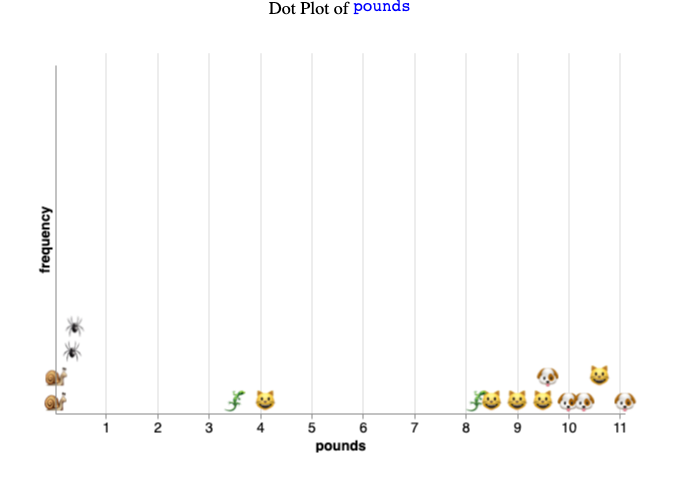
\includegraphics[width=0.48\textwidth]{images/320f755b0fe617c5.png}\hfill
    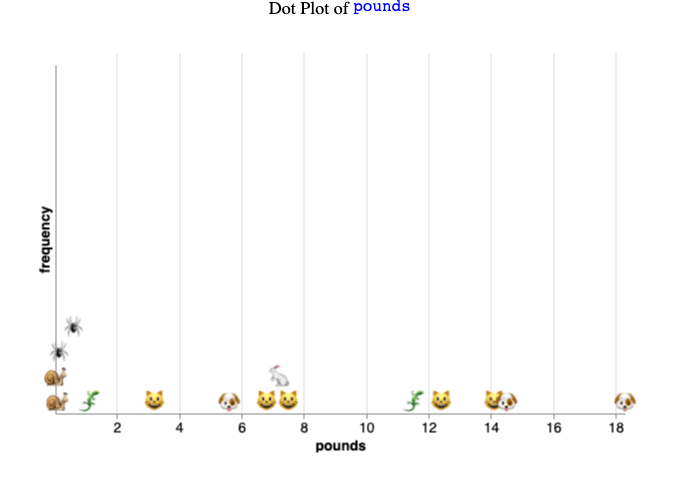
\includegraphics[width=0.48\textwidth]{images/c321846ad89322dc.png}
  \end{center}
  \begin{center}
    \small\emph{Dot plot du \texttt{poids} sur le jeu d'entraînement (gauche) et le jeu de test (droite). Chaque point est un emoji de l'espèce.}
  \end{center}
\end{thinkbox}

\begin{keypointbox}
  \textbf{Surapprentissage} (\emph{over-fitting})

  C'est un exemple de ce que les ingénieur·es en apprentissage automatique appellent le \textbf{surapprentissage}. Plus un classificateur dépend des particularités d'un attribut dans les données d'entraînement, plus il est sensible aux variations de cet attribut quand vient le moment d'utiliser de nouvelles entrées. Ici, \texttt{tree-q6} était \emph{totalement dépendant de seuils très spécifiques dans la colonne \texttt{poids}}, donc quand le jeu de test a eu des seuils différents, le classificateur a performé mal.

  \vspace{0.5em}
  Ce serait comme réviser pour un examen en mémorisant les réponses à un examen précédent. Vous avez appris à réussir \emph{ce test précis}, mais pas assez pour réussir un autre examen.

  \vspace{0.5em}
  En apprentissage automatique, le \textbf{surapprentissage} se produit quand notre arbre de décision essaie si fort de trouver un motif dans un ensemble spécifique de données qu'il commence à «~mémoriser~» les détails et le bruit aléatoire au lieu d'apprendre la règle réelle. C'est exactement ce qui s'est passé avec la colonne \texttt{poids} ici.

  Les autres colonnes ne variaient pas autant~! Les chiens et les chats sont tous des \texttt{mammiferes} quoi qu'il arrive. La plupart des chiens aiment \texttt{nager}. Et la plupart des chiens, chats et lézards ont une \texttt{queue}. Ces attributs sont plus stables entre les échantillons, alors que \texttt{poids} peut varier largement.
\end{keypointbox}

\subsection{Synthèse}

\begin{thinkbox}
  \begin{itemize}
    \item Expliquez comment la table du jeu de données d'entraînement est liée à l'arbre de décision.
    \begin{itemize}
      \item Les en-têtes de colonnes de la table sont les questions qui seront posées dans les nœuds de décision.
      \item Les données dans chaque colonne sont les réponses à ces questions, qui deviennent les étiquettes des arêtes de l'arbre («~oui~» et «~non~» pour ce jeu de données).
      \item Les catégories de sortie de la table sont les nœuds feuilles de l'arbre.
    \end{itemize}
    \item Un arbre de décision a-t-il généralement le même nombre de nœuds feuilles qu'il y a de lignes dans le jeu de données d'entraînement~? Pourquoi~?
    \begin{itemize}
      \item Non. L'algorithme de division fonctionne \emph{par attribut}~; en général, plusieurs lignes d'un jeu d'entraînement partagent des attributs. Donc, à moins que chaque ligne ait une combinaison unique d'attributs \emph{et} que l'arbre puisse aller infiniment profond, l'arbre aura moins de feuilles qu'il n'y a de lignes.
    \end{itemize}
    \item Un arbre de décision peut-il avoir \emph{moins} de nœuds feuilles qu'il n'y a de catégories uniques dans le jeu de données d'entraînement~? Pourquoi~?
    \begin{itemize}
      \item Oui. Un arbre peut ne pas être assez profond pour classifier correctement chaque catégorie — et dans certains cas, il peut ne \emph{pas y avoir} de façon de classifier correctement chaque catégorie~!
    \end{itemize}
  \end{itemize}
\end{thinkbox}

\newpage

% ===========================================================================
% SECTION 2 : ÉVALUER UN CLASSIFICATEUR
% ===========================================================================
\section{Évaluer un classificateur}

\begin{overviewbox}
  Les élèves découvrent les \textbf{matrices de confusion} et utilisent Pyret pour les générer à partir des fonctions classificateurs dérivées des arbres de décision.
\end{overviewbox}

% ---------- Launch ----------
\subsection{Lancement~: tests médicaux et classificateurs}

Les tests pour la grippe, la rougeole, etc. sont toutes des formes de classificateurs~! En examinant chacun de ces tests, les responsable·es de santé publique doivent penser aux cas suivants~:

\begin{center}
\begin{tabularx}{\textwidth}{l X X}
  \toprule
  \textbf{Statut réel} & \textbf{Prédit positif} & \textbf{Prédit négatif} \\
  \midrule
  Infecté       & \cellcolor{tp!15}\textcolor{tp}{\textbf{Vrai positif~:}} le test dit infecté, et la personne l'est \emph{réellement}
                & \cellcolor{fn!15}\textcolor{fn}{\textbf{Faux négatif~:}} le test dit infecté, mais la personne ne l'est pas \\[0.4em]
  Non infecté   & \cellcolor{fp!15}\textcolor{fp}{\textbf{Faux positif~:}} le test dit sain, mais la personne est malade
                & \cellcolor{tn!15}\textcolor{tn}{\textbf{Vrai négatif~:}} le test dit sain, et la personne l'est \emph{réellement} \\
  \bottomrule
\end{tabularx}
\end{center}

\begin{keypointbox}
  Il y a deux façons pour le test d'avoir \emph{raison}, et deux façons d'avoir \emph{tort}.

  Supposons que nous ayons une épidémie d'une maladie vraiment mortelle et hautement contagieuse, et deux tests possibles au choix~:
  \begin{itemize}
    \item \textbf{Test A} produit beaucoup de \emph{faux positifs}~: il fait presque toujours la bonne chose si vous êtes malade, mais beaucoup de personnes saines se font dire qu'elles sont infectées.
    \item \textbf{Test B} produit beaucoup de \emph{faux négatifs}~: il fait presque toujours la bonne chose si vous êtes sain·e, mais beaucoup de personnes malades se font dire qu'elles vont bien.
  \end{itemize}
\end{keypointbox}

\begin{thinkbox}
  Vous êtes ministre de la santé d'un pays qui subit une épidémie de cette maladie.
  \begin{itemize}
    \item Quel test choisissez-vous pour votre pays~?
    \item Choisiriez-vous un test différent pour une maladie \emph{moins} contagieuse~?
  \end{itemize}

  Laissez aux élèves le temps de discuter. Ce qui compte n'est pas que la classe aboutisse à une conclusion, mais que les élèves commencent à voir qu'il ne s'agit pas simplement de «~quelle est la précision du test~?~», mais plutôt «~dans quels cas le test se trompe-t-il, et combien de fois~?~».
\end{thinkbox}

\begin{keypointbox}
  Cet exemple concret montre clairement qu'il ne suffit pas de dire «~le classificateur avait raison la moitié du temps~».

  Sur les 5 chats du jeu de données, combien notre \texttt{classifieur-queue} a-t-il classifiés \emph{correctement}~?
  \begin{itemize}
    \item \textbf{5}. Soit $\approx 100\,\%$.
  \end{itemize}
  Sur les 2 tarentules, combien notre \texttt{classifieur-queue} a-t-il classifiées \emph{correctement}~?
  \begin{itemize}
    \item \textbf{0}. Soit $\approx 0\,\%$.
  \end{itemize}

  Les rapports que les data scientist·es (et les responsable·es de santé publique~!) utilisent pour comprendre à quel point un classificateur est «~bon~» s'appellent des \textbf{matrices de confusion}. Une matrice de confusion montre généralement des \emph{ratios}~:
  \begin{itemize}
    \item 0 sur 4 chiens devient $0\,\%$ (soit $0$ en décimal)
    \item 2 sur 2 lézards devient $100\,\%$ (soit $1$)
    \item 4 sur 5 chats devient $80\,\%$ (soit $0{,}8$)
  \end{itemize}
  …~et ainsi de suite.
\end{keypointbox}

% ---------- Investigate: hand-made confusion matrix ----------
\subsection{Construire une matrice de confusion à la main}

\begin{activitybox}
  Ajoutez ce classificateur à votre Zone de Définitions et cliquez sur «~Run~»~:
  \begin{lstlisting}
fun classifieur-nage(r):
  if r["nage"] == true:
    "chien"
  else:
    "chat"
  end
end
  \end{lstlisting}

  Avec votre voisin·e, utilisez la fonction \texttt{classify} pour remplir la matrice de confusion ci-dessous pour \texttt{classifieur-nage} sur le jeu \texttt{training}~:

  \vspace{0.5em}
  \begin{itemize}
    \item Remplissez d'abord le «~sur X~» (le nombre d'animaux de cette espèce dans le jeu).
    \item Convertissez ensuite le compte de prédictions correctes en \emph{pourcentage}.
    \item Enfin, convertissez le pourcentage en \emph{décimal}.
  \end{itemize}

  \vspace{0.5em}
  \begin{center}
  \small
  \begin{tabular}{l|c|c|c|c|c}
    \toprule
    \textbf{espece réelle} \textbackslash{} \textbf{prédit} & chat & chien & lezard & escargot & tarentule \\
    \midrule
    \texttt{"chat"}      & 4 sur 5 $= 80\,\% = 0{,}8$ & sur 5 & sur 5 & sur 5 & sur 5 \\
    \texttt{"chien"}     & sur 4 & sur 4 & sur 4 & sur 4 & sur 4 \\
    \texttt{"lezard"}    & sur 2 & sur 2 & sur 2 & sur 2 & sur 2 \\
    \texttt{"escargot"}  & sur 2 & sur 2 & sur 2 & sur 2 & sur 2 \\
    \texttt{"tarentule"} & sur 2 & sur 2 & sur 2 & sur 2 & sur 2 \\
    \bottomrule
  \end{tabular}
  \end{center}
\end{activitybox}

\img{images/b74bc727477a4c35.png}{width=0.65\textwidth}{Capture d'écran d'une matrice de confusion Pyret pour le \texttt{classifieur-nage}, évaluée sur le jeu de données d'entraînement.}

\begin{thinkbox}
  \begin{itemize}
    \item Quelle espèce \texttt{classifieur-nage} a-t-il prédite le \emph{plus} précisément~?
    \begin{itemize}
      \item Les chiens.
    \end{itemize}
    \item Quelle espèce a-t-il prédite le \emph{moins} précisément~?
    \begin{itemize}
      \item Les escargots, les lézards et les tarentules.
    \end{itemize}
    \item Qu'apprend-on d'autre de la matrice de confusion~?
    \begin{itemize}
      \item Tous les escargots et tarentules sont mal classifiés en chats.
      \item La moitié des lézards sont mal classifiés en chats, l'autre moitié en chiens.
      \item 20\,\% des chats sont mal classifiés en chiens.
    \end{itemize}
  \end{itemize}
\end{thinkbox}

% ---------- Investigate: Pyret confusion matrix ----------
\subsection{Laisser Pyret construire la matrice}

Pyret possède une fonction qui construit une matrice de confusion pour vous~! Voici le contrat~:

\contrat{\# confusion-matrix :: (Table t, String colonne-reponse, (Row -> String) classifieur) -> Table}

\begin{activitybox}
  Testez la matrice de confusion pour notre \texttt{classifieur-nage} avec le code suivant~:
  \begin{lstlisting}
confusion-matrix(training, "espece", classifieur-nage)
  \end{lstlisting}

  \begin{enumerate}[leftmargin=*]
    \item Comparez la matrice que vous avez faite à la main avec celle produite par Pyret. Si elles ne correspondent pas, travaillez avec votre voisin·e pour comprendre pourquoi.
    \item Générez une matrice de confusion pour \texttt{classifieur-nage} sur la table \texttt{testing}. Que remarquez-vous~? Comment la performance sur \texttt{testing} se compare-t-elle à celle sur \texttt{training}~?
    \begin{itemize}
      \item Iel s'en sort très bien, mais mal classifie tous les lapins en chiens.
      \item On ne s'attendrait pas à ce qu'il classifie correctement l'espèce d'un animal sur lequel il ne s'est pas entraîné.
    \end{itemize}
    \item Construisez une matrice de confusion pour notre \texttt{classifieur-queue} original et préparez-vous à partager ce que vous apprenez.
  \end{enumerate}
\end{activitybox}

\subsubsection{Lire une matrice de confusion}

\begin{keypointbox}
  Voici la matrice de confusion pour \texttt{classifieur-queue} sur le jeu d'entraînement~:

  \vspace{0.4em}
  \begin{center}
  \small
  \begin{tabular}{l|c|c|c|c|c}
    \toprule
    \textbf{espece réelle} \textbackslash{} \textbf{prédit} & chat & chien & lezard & escargot & tarentule \\
    \midrule
    \texttt{"chat"}      & \cellcolor{tp!20}\textbf{1} & 0 & 0 & 0 & 0 \\
    \texttt{"chien"}     & 1 & \cellcolor{tp!20}\textbf{0} & 0 & 0 & 0 \\
    \texttt{"lezard"}    & 1 & 0 & \cellcolor{tp!20}\textbf{0} & 0 & 0 \\
    \texttt{"escargot"}  & 0 & 0 & 0 & \cellcolor{tp!20}\textbf{1} & 0 \\
    \texttt{"tarentule"} & 0 & 0 & 0 & 1 & \cellcolor{tp!20}\textbf{0} \\
    \bottomrule
  \end{tabular}
  \end{center}

  \vspace{0.3em}
  Les «~bons scores~» apparaissent sur la \textbf{diagonale}, du coin supérieur gauche au coin inférieur droit. \textbf{Note~: nous utilisons des valeurs entre 0 et 1, plutôt que des pourcentages~!} «~80\,\%~» apparaîtrait comme \texttt{0.8}.
\end{keypointbox}

\begin{thinkbox}
  \begin{itemize}
    \item Que pouvons-nous déduire de cette matrice de confusion~?
    \begin{itemize}
      \item Le classificateur a 100\,\% des chats et des escargots corrects.
      \item Iel a mal classifié tous les chiens en chats.
      \item Iel a mal classifié tous les lézards en chats.
      \item Iel a mal classifié toutes les tarentules en escargots.
    \end{itemize}
    \item À quoi ressemblerait la matrice pour le \textbf{meilleur classificateur possible}~?
    \begin{itemize}
      \item Des 1 sur la diagonale, montrant~:
      \begin{itemize}
        \item 100\,\% des chats prédits en chats
        \item 100\,\% des chiens prédits en chiens
        \item 100\,\% des lézards prédits en lézards
        \item …~etc.
      \end{itemize}
      \item Des 0 partout ailleurs, montrant qu'il n'y a pas de mauvaises classifications.
    \end{itemize}
  \end{itemize}
\end{thinkbox}

% ---------- Synthesize ----------
\subsection{Synthèse}

\begin{thinkbox}
  \begin{itemize}
    \item Pourquoi un arbre de décision précis à 100\,\% sur les données d'entraînement ne fait-il pas toujours de bonnes prédictions sur les données de test~?
    \begin{itemize}
      \item Si le classificateur est surajusté (\emph{overfit}) aux données d'entraînement, il pourrait ne pas faire de bonnes prédictions sur des données liées mais différentes.
      \item Les modèles basés sur des colonnes quantitatives sont particulièrement sensibles au surapprentissage.
    \end{itemize}
    \item Avec vos propres mots, décrivez ce qu'est une matrice de confusion.
  \end{itemize}
\end{thinkbox}

\begin{keypointbox}
  \emph{Tous les modèles se trompent. Certains sont utiles.}

  \vspace{0.4em}
  \begin{itemize}
    \item Quand un arbre de décision se trompe-t-il~?
    \item Quand est-il utile~?
  \end{itemize}
\end{keypointbox}

\newpage

% ===========================================================================
% ANNEXES
% ===========================================================================
\section*{Annexe A~: Visualiser le surapprentissage}

Les \emph{dot plots} ci-dessous comparent la distribution du \texttt{poids} entre le jeu d'entraînement et le jeu de test. Chaque point est un emoji de l'espèce de l'animal~: chat, chien, lézard, escargot, tarentule, et (dans le jeu de test) lapin. Les emojis exacts sont visibles sur les dot plots ci-dessous.

\begin{center}
  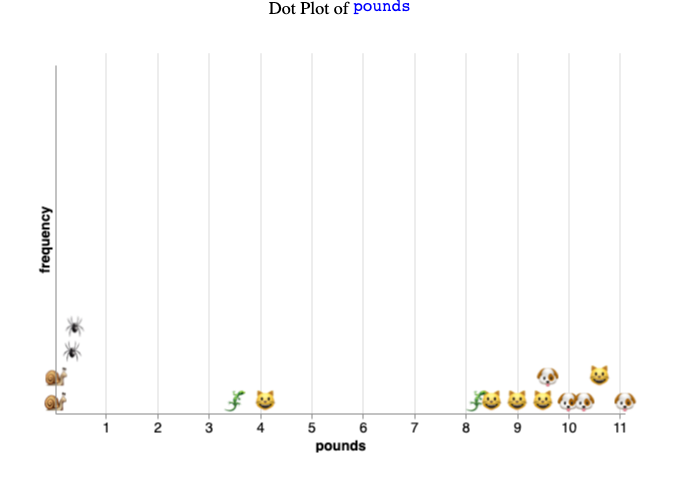
\includegraphics[width=0.48\textwidth]{images/320f755b0fe617c5.png}\hfill
  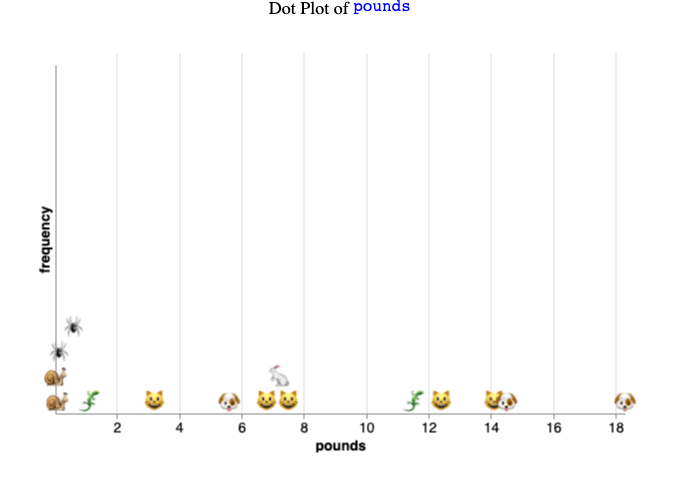
\includegraphics[width=0.48\textwidth]{images/c321846ad89322dc.png}
\end{center}
\begin{center}
  \small\emph{Gauche~: jeu d'entraînement (chats, chiens, lézards, escargots, tarentules). Droite~: jeu de test (mêmes espèces + lapins).}
\end{center}

\subsection*{Pourquoi \texttt{tree-q6} se trompe-t-il sur le jeu de test~?}

L'arbre \texttt{tree-q6} a été construit en utilisant \emph{uniquement} la colonne \texttt{poids} avec une profondeur maximale de 6~niveaux. Sur le jeu d'entraînement, il a trouvé des seuils \emph{parfaits} qui séparent chaque espèce. Mais ces seuils sont très spécifiques~: par exemple, «~\texttt{poids < 9{,}55}~» sépare les chats des chiens dans \emph{ce} jeu d'entraînement, mais un chat plus lourde qu'un chien dans le jeu de test sera mal classifié.

\begin{center}
\begin{tikzpicture}[
  level 1/.style={sibling distance=4.5cm, level distance=1.5cm},
  level 2/.style={sibling distance=2.2cm, level distance=1.5cm},
  level 3/.style={sibling distance=1.6cm, level distance=1.3cm},
  every node/.style={align=center},
  edge from parent/.style={draw, thick, ->, >=Stealth},
]
\node[root] {poids < 9.55~?}
  child {
    node[decision] {poids < 0.19~?}
    child {
      node[leaf] {escargot}
      edge from parent node[left, font=\scriptsize\bfseries, text=bsgreen] {oui}
    }
    child {
      node[decision] {poids < 1.95~?}
      child {
        node[leaf] {tarentule}
        edge from parent node[left, font=\scriptsize\bfseries, text=bsgreen] {oui}
      }
      child {
        node[leaf] {chat}
        edge from parent node[right, font=\scriptsize\bfseries, text=bsorange] {non}
      }
      edge from parent node[right, font=\scriptsize\bfseries, text=bsorange] {non}
    }
    edge from parent node[left, font=\scriptsize\bfseries, text=bsgreen] {oui}
  }
  child {
    node[leaf] {chien}
    edge from parent node[right, font=\scriptsize\bfseries, text=bsorange] {non}
  };
\end{tikzpicture}
\end{center}

\vspace{0.5em}
\textbf{L'arbre \texttt{tree-q3} ci-dessus est parfait sur le jeu d'entraînement, mais se trompe sur le jeu de test dès qu'un animal a un poids inattendu. C'est le surapprentissage.}

\section*{Annexe B~: Fichiers du projet}

\begin{center}
\begin{tabularx}{\textwidth}{l X}
  \toprule
  \textbf{Fichier} & \textbf{Description} \\
  \midrule
  \texttt{Arbre\allowbreak-Decision\allowbreak-Starter.arr} & Fichier de démarrage Pyret (inchangé par rapport à la leçon précédente). Fournit \texttt{build-tree}, \texttt{confusion-matrix}, \texttt{classify}, \texttt{dt-code}, etc. via \texttt{ai-library.arr}. \\
  \texttt{evaluer-arbres-decision.tex} & Document de cours (ce fichier) \\
  \texttt{images/320f755b0fe617c5.png} & Dot plot du \texttt{poids}, jeu d'entraînement \\
  \texttt{images/c321846ad89322dc.png} & Dot plot du \texttt{poids}, jeu de test (avec lapins) \\
  \texttt{images/b74bc727477a4c35.png} & Capture d'écran d'une matrice de confusion Pyret \\
  \texttt{images/CCbadge.png} & Logo Creative Commons \\
  \bottomrule
\end{tabularx}
\end{center}

\vspace{1em}
\textbf{À noter~:} cette leçon utilise \emph{le même} fichier \texttt{Arbre-Decision-Starter.arr} que la leçon précédente (Construire des arbres de décision). Aucune modification du code n'est nécessaire~: \texttt{build-tree}, \texttt{confusion-matrix}, \texttt{dt-code}, \texttt{classify} sont fournis par la bibliothèque \texttt{ai-library.arr} de Bootstrap, chargée via \texttt{use context url-file(...)}.

\section*{Annexe C~: Pour aller plus loin}

\begin{instructornotes}
  \textbf{Bientôt disponible~!}

  Vous voulez que vos élèves pratiquent leurs compétences et appliquent leurs connaissances des classificateurs à des données du monde réel~? Faites-leur ouvrir le \emph{AI Music Starter File} de Bootstrap (\url{https://pyret.BootstrapWorld.org/editor\#shareurl=https://raw.githubusercontent.com/bootstrapworld/starter-files/refs/heads/main/ai/ai-music.arr}) et construire un arbre de décision capable de différencier les chansons R\&B, Rock'n'Roll et Country~! Le fichier de démarrage est prêt aujourd'hui~; nous mettrons à jour la page du cahier d'exercices et ajouterons une section optionnelle à cette leçon qui structure l'ensemble.
\end{instructornotes}

\section*{À propos de ces supports}

Ces supports ont été développés en partie grâce au soutien de la \emph{National Science Foundation} (bourses 1042210, 1535276, 1648684, 1738598, 2031479 et 1501927).

\begin{center}
  \textbf{Bootstrap} par la Communauté Bootstrap est sous licence Creative Commons 4.0 Unported.\\
  Cette licence n'accorde pas la permission d'organiser des formations ou du développement professionnel.\\[1em]
  \textit{Traduction et adaptation française réalisées en juillet 2026.}\\
  \textit{Source originale~: \url{https://www.bootstrapworld.org/materials/fall2026/en-us/lessons/decision-trees-evaluating/}}
\end{center}

\end{document}